\documentclass[conference]{IEEEtran}
\IEEEoverridecommandlockouts
% The preceding line is only needed to identify funding in the first footnote. If that is unneeded, please comment it out.
\usepackage[french]{babel}
\usepackage[utf8]{inputenc}
\usepackage[T1]{fontenc}
\usepackage{cite}
\usepackage{amsmath,amssymb,amsfonts}
\usepackage{algorithmic}
\usepackage{graphicx}
\usepackage{textcomp}
\usepackage[babel=true]{csquotes}
\usepackage{pgf,tikz}
\usepackage{listings}
\usepackage{xcolor}

\usetikzlibrary{shapes}
\usetikzlibrary{arrows}
\tikzset{
  font={\fontsize{7pt}{12}\selectfont}}
\usetikzlibrary{graphs}

\def\BibTeX{{\rm B\kern-.05em{\sc i\kern-.025em b}\kern-.08em
    T\kern-.1667em\lower.7ex\hbox{E}\kern-.125emX}}
 
\definecolor{codegreen}{rgb}{0,0.6,0}
\definecolor{codegray}{rgb}{0.5,0.5,0.5}
\definecolor{codepurple}{rgb}{0.58,0,0.82}
\definecolor{backcolour}{rgb}{0.95,0.95,0.92}
 
\lstdefinestyle{mystyle}{
    backgroundcolor=\color{backcolour},   
    commentstyle=\color{codegreen},
    keywordstyle=\color{magenta},
    numberstyle=\tiny\color{codegray},
    stringstyle=\color{codepurple},
    basicstyle=\ttfamily\footnotesize,
    %breakatwhitespace=false,         
    breaklines=true,                 
    captionpos=t,                    
    keepspaces=true,                 
    numbers=left,                    
    numbersep=5pt,                  
    showspaces=false,                
    showstringspaces=false,
    showtabs=false,                  
    tabsize=2,
    breaklines=true,
    literate=%
	{á}{{\'a}}1 {à}{{\`a}}1 {í}{{\'i}}1 {é}{{\'e}}1 {è}{{\`e}}1 {ý}{{\'y}}1 {ú}{{\'u}}1
	{ó}{{\'o}}1 {ô}{{\^o}}1 {ě}{{\v{e}}}1 {š}{{\v{s}}}1 {č}{{\v{c}}}1 {ř}{{\v{r}}}1
	{ž}{{\v{z}}}1 {ď}{{\v{d}}}1 {ť}{{\v{t}}}1 {ň}{{\v{n}}}1 {ů}{{\r{u}}}1 {Á}{{\'A}}1
	{Í}{{\'I}}1 {É}{{\'E}}1 {Ý}{{\'Y}}1 {Ú}{{\'U}}1 {Ó}{{\'O}}1 {Ě}{{\v{E}}}1
	{Š}{{\v{S}}}1 {Č}{{\v{C}}}1 {Ř}{{\v{R}}}1 {Ž}{{\v{Z}}}1 {Ď}{{\v{D}}}1 {Ť}{{\v{T}}}1
	{Ň}{{\v{N}}}1                {Ů}{{\r{U}}}1
}
 
\lstset{style=mystyle}


\begin{document}

\title{Simulation d'une voiture autonome sur le RTOS QNX}

\author{\IEEEauthorblockN{Antonin Godard (2032402)}
\IEEEauthorblockA{\textit{Génie Informatique} \\
\textit{Polytechnique Montréal}\\
Montréal, Québec \\
antonin.godard@polymtl.ca}
\and
\IEEEauthorblockN{Rayan Neggazi (2038882)}
\IEEEauthorblockA{\textit{Génie Informatique} \\
\textit{Polytechnique Montréal}\\
Montréal, Québec \\
rayan.neggazi@polymtl.ca}
}

\maketitle

\begin{abstract}

Cet article présente la simulation d'une voiture
autonome sur un système d'exploitation temps-réel
 QNX (Blackberry). Cette voiture se déplace sur un terrain
 supposé plat, où elle doit atteindre une destination 
 finale en passant par plusieurs étapes. Elle doit également
 prendre en compte des obstacles générés aléatoirement sur sa
 trajectoire.
 
 L'étude se focalise sur la modélisation de la partie continue ainsi que la partie
 discrète du système. Il ne s'agit donc en aucun cas d'étudier les mécaniques de la
 voiture ou l'électronique des composants. L'article porte sur la modélisation de la
 partie \enquote{intelligente} du système et principalement trois entités :
 \begin{itemize}
     \item le contrôle de la destination de la voiture ;
     \item le contrôle de la navigation de la voiture ;
     \item le contrôle de la caméra de la voiture.
 \end{itemize}
 
 Cet article montre les différentes techniques de parallélisation
 de tâches ainsi qu'un exemple de partitionnement CPU de ces dernières. On parlera aussi des cas d'utilisation ajoutés au système en vue de son amélioration.
 
 Il y figure également les problèmes rencontrés ainsi que les solutions apportées et les résultats associés à ces solutions.
 
\end{abstract}

\begin{IEEEkeywords}
simulation, RTOS, QNX, partion\-nement, modé\-lisation
\end{IEEEkeywords}

%\tableofcontents

\section{Introduction}

La voiture autonome a été premièrement analysée et décrite avec les différentes normes UML. Nous avons choisi de réaliser quatre diagrammes (voir Annexe) :
\begin{itemize}
    \item un diagramme de cas d'utilisation afin de décrire dans quel contexte évolue le système;
    \item un diagramme de séquence qui décrit le comportement du système dans le temps;
    \item un organigramme décrivant la partie logique du système \item un diagramme d'objets pour décrire la structure de la voiture.
\end{itemize}{}
 
Ces quatre diagrammes nous ont permis d'établir une vision claire du système afin de passer à la modélisation et à la simulation.

Dans un premier temps, nous avons réalisé une modélisation avec TrueTime, un simulateur s'exécutant sur MatLab et Simulink. Dans cette partie, nous avons réalisé la partie \emph{discrète} du système -- c'est à dire la modélisation du comportement de la voiture. Cette partie discrète envoie des commandes à la partie continue et de cette façon nous contrôlions la voiture (sa vitesse, son orientation, et la prise de photo).

Dans un second temps, nous sommes passé à la simulation de la voiture sur une autre plateforme : le RTOS QNX, développé par Blackberry. Ce système d'exploitation temps-réel permet l'implantation de systèmes temps-réels avec l'utilisation de mécanismes sophistiqués régis par la norme POSIX.

Cette simulation s'est effectuée en deux temps :
\begin{enumerate}
    \item une modélisation purement fonctionnelle de la voiture ayant pour objectif de répondre au cahier des charges préalablement fourni
    \item une amélioration du modèle ainsi que l'ajout de méca\-nismes propres à QNX
\end{enumerate}

Ainsi, l'article portera sur la dernière partie de la modé\-lisation sur QNX. On parlera des problèmes rencontrés, des solutions proposées et des résultats obtenus afin d'obtenir un système performant.

Pour modéliser la voiture, nous avons séparé les diffé\-rentes fonctions de la voiture en tâches qui communiquent à travers des variables. Chaque tâche est en fait un fil d'exécution de la bibliothèque \texttt{pthread}. Tout ces fils sont initialisés au même instant et ont chacun un second fil associé représentant leur timer, et donc leur périodicité.

Plus précisément, chaque tâche de la voiture a une routine infinie associée, qui est lancée depuis une routine principale nommée \texttt{main\_worker} qui leur est toute commune. Ce choix d'avoir une routine commune à chaque fil qui vient lancer une routine spécifique en fonction du fil rend le code plus lisible mais surtout plus modulaire. Il nous était donc facile de modifier les caractéristiques d'une tâche (période, priorité), d'en ajouter ou d'en supprimer.

La séparation des tâches respecte la description initiale de notre système. Les tâches continues et discrètes ont chacune un fil d'exécution associé. Nous avons ajouté une tâche d'affichage (display), deux tâches de détection de niveau de batterie (faible et élevé), et une tâche de trace de données, sur laquelle nous reviendrons dans la section~\ref{sec:ameliorations}.



\section{Lacunes de la première implantation}

\subsection{Incertitude de la périodicité des tâches}

Chaque tâche dans notre programme a besoin d'être exécutée de manière périodique, avec des périodes différentes évidemment. Afin de remplir cette fonction, nous avons initialement intégré des instructions de type \enquote{sleep} dans chaque tâche avec le temps pendant lequel nous souhaitions endormir notre programme.

Toutefois, les tâches n'étaient pas réveillées de de manière précise a chaque intervalle de temps indiqué par l'instruction sleep en question. En effet, le programme s'endort bien pour cette période mais seulement après avoir exécuté toutes les autres instructions qui le composent. Ainsi, la période réelle de la tâche est le temps de consigne du sleep auquel il faut ajouter le temps d'exécution de l'ensemble du programme qui de plus, varie d'un appel à l'autre en fonction des conditions et des paramètres actualisés.

\subsection{Variables globales pour la synchronisation}

Étant donné la nécessité de communiquer entre les parties \emph{opérative} et \emph{contrôle} notamment, nous avons ,dans un premier temps, fait le choix d'utiliser des variables globales. 

Cependant, cette méthode ne garantissait ni un accès optimal aux variables partagées, ni une synchronisation parfaite entre les threads de contrôle et d'opération.

\subsection{Temps de simulation}

Après avoir terminé la modélisation de base de la voiture, la simulation fonctionnait mais elle ne pouvait être accélérée.

La simulation se réalisait en temps réel comme si la voiture avançait réellement à 30 ou 50km/h. Il fallait attendre trop longtemps pour que la voiture atteigne un nombre signifiant d'étapes, de stations et de destinations. De plus, la batterie se déchargeait trop lentement.

%\subsection{Priorités des tâches}

\section{Solutions et améliorations proposées}
\label{sec:ameliorations}

\subsection{Solutions aux lacunes}

\subsubsection{Ajout de timers}

Afin de corriger cette erreur causée par l'utilisation de la fonction sleep dans nos tâches, nous avons remplacé ces derniers par des timers. Les fonctions nécessaires à cet objectif ont été extraites d'un code fourni, et intégrées à part dans un fichier timers.cpp. 

Ainsi, pour chaque tâche nous avons initialisé un timer (grâce à la fonction init\_timer) prenant en paramètre notamment la période désirée, ainsi qu'un pulse handler (à l'aide de la fonction task\_pulse\_handler). Celui-ci permet alors de réveiller la tâche en question à chaque période par l'utilisation d'une sémaphore. Le thread, pour être exécuté doit désormais attendre que sa sémaphore soit relâchée par son pulse handler.

\subsubsection{Synchronisation des tâches aves des sémaphores}

Pour exécuter les fils périodiquement nous utilisons un fil associé à chaque thread qui modélise un timer. Ce fil vient périodiquement relâcher une sémaphore sur laquelle chaque tâche attend. Ces sémaphores nommées \texttt{sync\_sem} font partie de la structure de données passées à chacune des tâches.

Pour la synchronisation de la partie contrôle de la caméra, nous utilisons également une sémaphore pour \enquote{réveiller} la partie continue de la caméra tous les 10 mètres. Deux sémaphores sont aussi utilisées pour réveiller les deux fils associés à la détection de batterie haute et faible.

\subsubsection{Accélération de la simulation}

Pour palier au problème de temps de simulation, nous avons ajouté un macro \texttt{SIMU\_ACCEL} nous permettant d'ajuster la vitesse de simulation. Ce facteur vient jouer sur plusieurs paramètres :
\begin{itemize}
    \item augmenter le pas d'avancement de la voiture ;
    \item accélérer la décharge la batterie ;
    \item multiplier le temps de trace de données pour avoir une estimation du temps réel écoulé.
\end{itemize}

Cependant, accélérer la simulation veut aussi dire qu'il faut ajuster la période des tâches ayant besoin de précision. Nous avons notamment rencontré un problème lors de la détection à moins de dix mètres.

Ainsi, les tâches de contrôle ont une fréquence bien supérieure aux tâches continues.

\subsection{Améliorations}

\subsubsection{Utilisation raisonnable de mutex}

Il nous a semblé important d'utiliser le strict minimum en terme de mutex car ce sont des mécanismes utilisant beaucoup de ressources. Ainsi, nous en utilisons 4 pour les 4 données physiques de la voiture : vitesse, angle, niveau de batterie, et position courante. Nous pensons que cela est un bon compromis entre le nombre de mutex utilisés et la granularité des accès. 

En effet, nous aurions pu n'utiliser qu'une seule mutex pour les quatre données (toutes stockées dans la même structure) mais cela aurait bloqué trop de tâches.

\subsubsection{Trace de données}

Garder un historique des données de la voiture nous semblait être une bonne amélioration étant donné qu'en réalité les logs sont indispensables au débogage. Nous avons alors ajouté un fil d'exécution qui écrit périodiquement le données de la voiture dans un fichier toutes les 100ms.

Cette amélioration est également utile afin de montrer les résultats obtenus, dont nous discutons section~\ref{sec:resultats}. On peut notamment voir l'évolution de la vitesse et de la batterie en fonction de la position et du temps.

Le code servant à tracer les données se trouve en annexe.

\subsubsection{Ajout d'obstacles devant la voiture}

Pour le contrôle de la navigation, nous avions décidé de modéliser le comportement de la voiture par une machine à états, car cela augmente la modularité de l'implantation, et permet une meilleure compréhension du comportement.

Ainsi le résultat que nous avons obtenu est celui de la figure~\ref{fig:state_machine_1}. 
L'état \texttt{GOTO\_DEST} représente l'état initial de la voiture, où elle doit se diriger vers la prochaine étape. L'état \texttt{PRE\_BATTLOW} survient lorsque la batterie est faible, met la vitesse de la voiture à 30km/h et détermine la station la plus proche. L'état \texttt{BATTLOW} fait en sorte de déterminer si la voiture est arrivée à la station. Lors de l'arrivée la voiture passe à l'état \texttt{CHARGING}, qui représente la recharge de la voiture. Finalement la voiture retourne à l'état initial lorsque la batterie est chargée.

Mais nous nous placions également dans une situation réelle où il est possible que la voiture rencontre des obstacles -- que ce soit lorsqu'elle se rend à une étape ou à une station. Ainsi, nous avons ajouté deux états à la machine afin de modéliser cet ajout.

La génération d'obstacle est aléatoire et s'exécute à chaque fois que la voiture atteint une étape. L'obstacle sera, avec une probabilité prédéfinie, positionné à une distance elle aussi aléatoire entre la voiture et la prochaine étape.

L'état \texttt{PRE\_OBSTACLE} est alors atteint quand la voiture arrive à 5 mètres de l'obstacle. Cet état met la vitesse de la voiture à 0 et démarre un timer. En fait, en réalité, cette fonction de la voiture serait un capteur qui détecte et met en arrêt d'urgence la voiture lorsque une personne ou un objet est devant.

L'état \texttt{OBSTACLE} attend que le timer soit écoulé, puis fait repartir la voiture. Nous aurions pu modéliser cela de plusieurs façons mais nous avons jugé le timer suffisant. Également, cet état doit prendre compte la variable \texttt{lowBat}, représentant l'état de la batterie faible, pour retourner au bon état.

\begin{figure}[h]
    \centering
    \begin{tikzpicture}[scale = 1]
    
    \tikzset{edge/.style = {->,> = latex'}}
    
    % vertices
    \node[rounded corners=3pt, draw=black, rectangle split, rectangle split parts = 2] (a) at  (-2,0) {\texttt{GOTO\_DEST} \nodepart{two} {\tiny vit. = 50km/h}};
    \node[rounded corners=3pt, draw=black, rectangle split, rectangle split parts = 2] (b) at  (2,0) {\texttt{PRE\_BATTLOW}\nodepart{two} {\tiny vit. = 30km/h}};
    \node[rounded corners=3pt, draw=black, rectangle split, rectangle split parts = 2] (c) at  (2,2) {\texttt{BATTLOW}\nodepart{two} {\tiny vit. = 30km/h}};
    \node[rounded corners=3pt, draw=black, rectangle split, rectangle split parts = 2] (d) at  (-2,2) {\texttt{CHARGING}\nodepart{two} {\tiny vit. = 0km/h}};
    \node[rounded corners=3pt, draw=black, rectangle split, rectangle split parts = 2] (e) at  (0,-2) {\texttt{PRE\_OBSTACLE}\nodepart{two} {\tiny vit. = 0km/h}};
    \node[rounded corners=3pt, draw=black, rectangle split, rectangle split parts = 2] (f) at  (0,-4) {\texttt{OBSTACLE}\nodepart{two} {\tiny vit. = 0km/h}};
    \node[circle, fill=black] (g) at (0,1) {};
    
    %edges
    \draw[edge] (g) to node [] {} (a);
    \draw[edge] (a) to node [above] {batt = 10} (b);
    \draw[edge] (b) to node [left] {} (c);
    \draw[edge] (c) to node [above] {closeTo(station)} (d);
    \draw[edge] (d) to node [left] {batt = 80} (a);
    \draw[edge] (a) to node [sloped, above] {\tiny closeTo(obstacle)} (e);
    \draw[edge] (b) to node [sloped, above] {\tiny closeTo(obstacle)} (e);
    \draw[edge] (e) to node [left] {} (f);
    \draw[edge] (f) to[bend left = 25] node [left] {!lowBat} (a);
    \draw[edge] (f) to[bend right = 25] node [right] {lowBat} (b);
    
    \end{tikzpicture}
    \caption{Contrôle de la navigation avec obstacle}
    \label{fig:state_machine_1}
\end{figure}

\subsubsection{Partitionnement CPU des tâches}

Un des mécanismes de QNX que nous avons choisi est le partitionnement des tâches. QNX propose un partitionnement \textit{adaptatif} qui permet l'assignation de tâches dynamiquement, après leur création. Le partitionnement est un point critique des systèmes temps-réel ayant besoin d'un haut niveau de sûreté. Cela permet notamment de diviser les tâches en groupes et de définir un \textit{pourcentage} de temps CPU alloué à la partition.

Nous avons choisi de diviser les tâches continues et les tâches discrètes dans des partitions séparées car ce sont deux corps de tâches avec un fonctionnement différent. Cela se justifie également par l'aspect sécuritaire que le partitionnement ajoute : il limite l'usage des ressources CPU, ce qui empêche une partition gourmande de prendre toutes les ressources et de bloquer les autres tâches dans les autres partitions.

Nous avons choisi de limiter la partie continue à 20\% ainsi que la partie discrète à 60\%.



\section{Résultats}
\label{sec:resultats}

Pour cette section, nous nous baserons sur une seule et même exécution de la simulation.

\subsection{Accélération de la simulation}

L'accélération de la simulation a bien fonctionné. Comme peut en témoigner l'analyse de photo figure~\ref{fig:path_image}, on atteint bien deux étapes et une station.

\begin{figure}
    \centering
    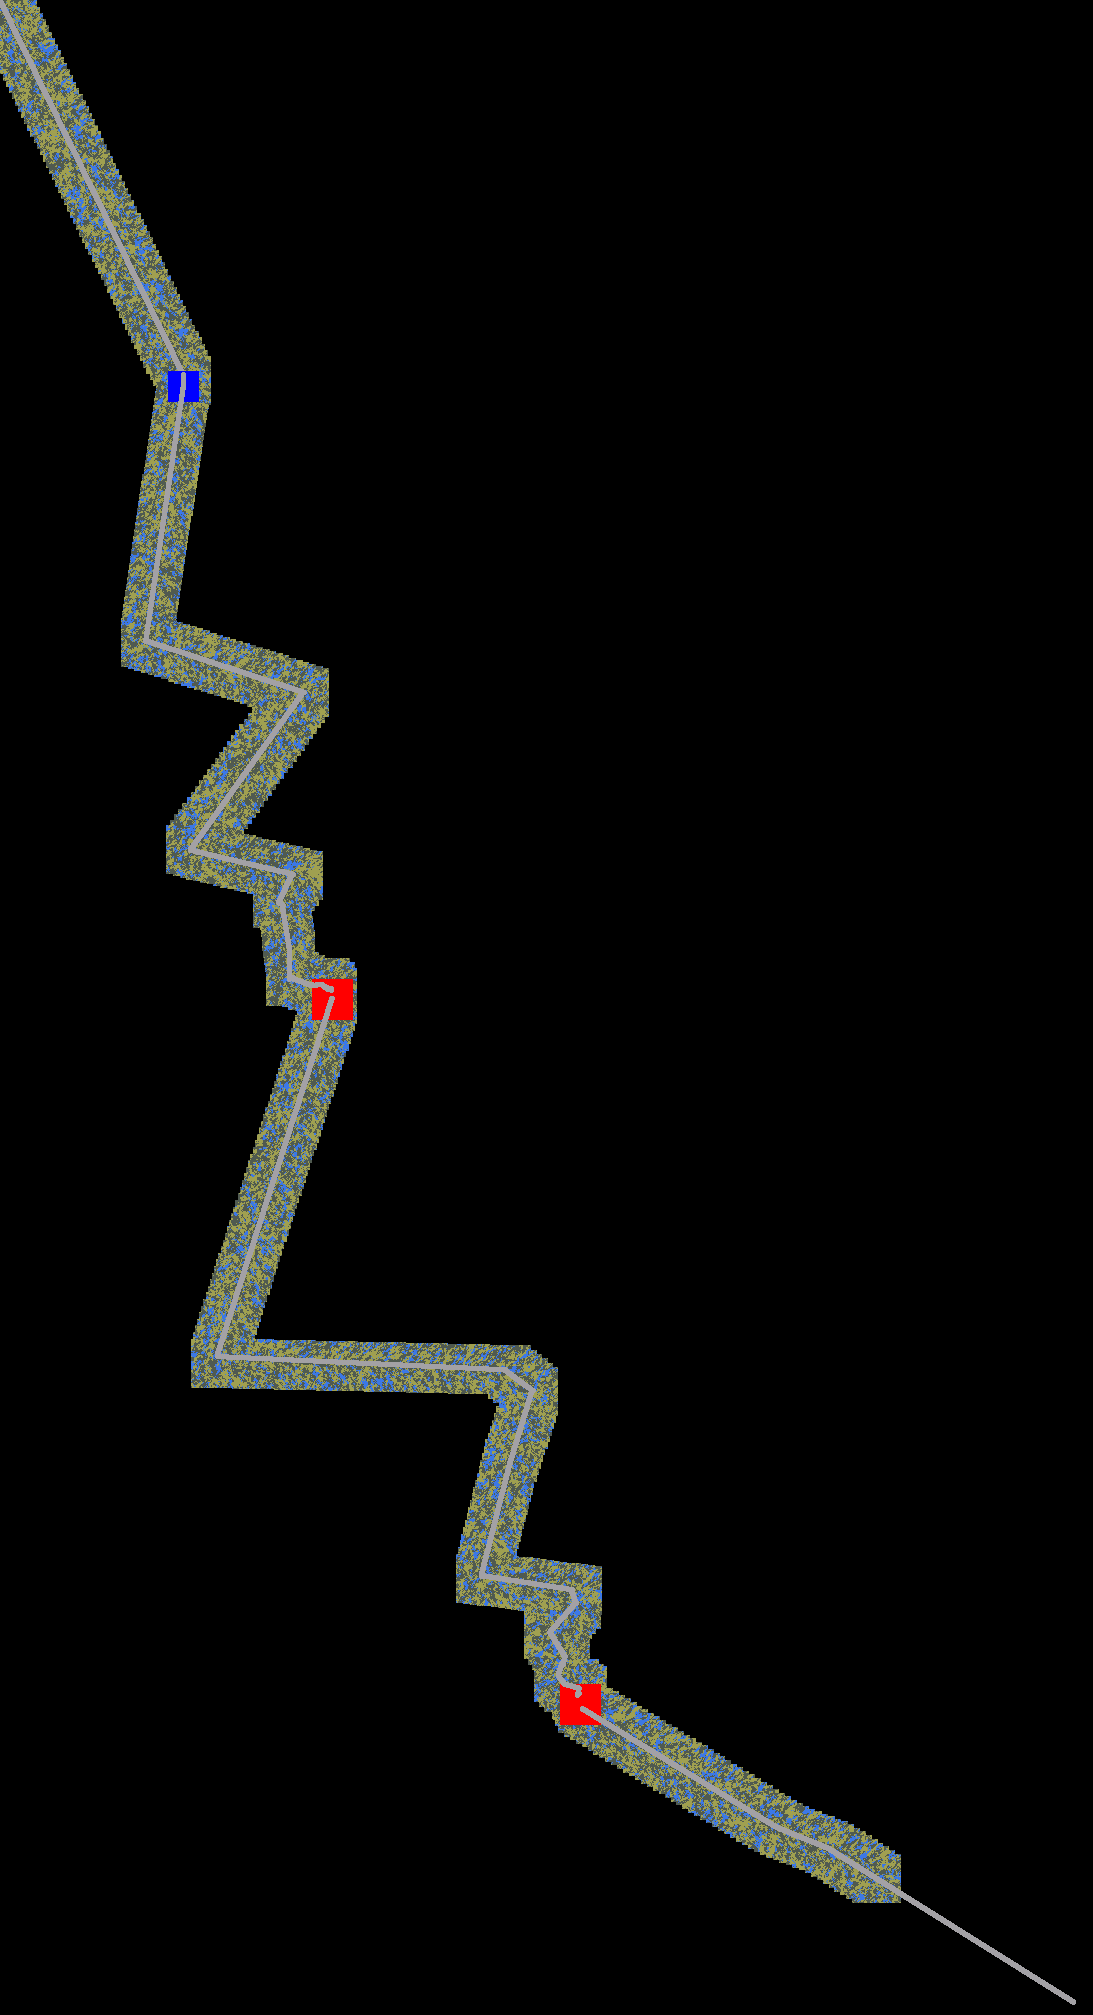
\includegraphics[height=0.7\linewidth]{map.png}
    \caption{Tracé avec \texttt{takePhoto}}
    \label{fig:path_image}
\end{figure}

\subsection{Trace des données de la voiture et analyse graphique}

On peut observer le déplacement de la voiture figure~\ref{fig:path}. Nous nous sommes limités à l'affichage des deux premières étapes pour améliorer la lisibilité. La légende indique les points importants du graphique, et la barre de couleur indique l'état de la batterie à un point donné.

On peut donc confirmer que la voiture est bien chargée après le départ d'une station, et que la voiture effectue bien son chemin étape par étape jusqu'à la destination finale.

On remarque aussi qu'une étape proche de la station n'est pas atteinte. Cela s'explique pqr le fait que la voiture régénère une étape après être chargée.

La figure~\ref{fig:speed} montre l'évolution de la vitesse pendant la simulation. On voit que la voiture est à 30km/h pendant un bref instant pour aller à la station. On voit également que la voiture s'arrête pendant un instant lorsqu'elle détecte un obstacle.

\begin{figure}[h]
    \centering
    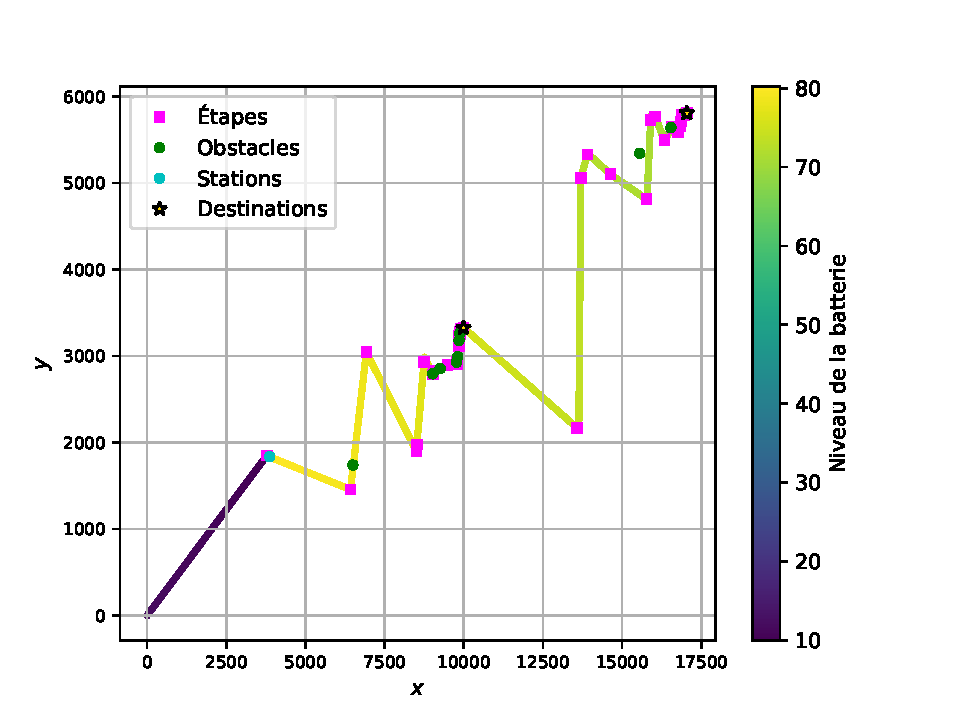
\includegraphics[width=1.1\linewidth]{path.pdf}  
    \caption{Chemin de la voiture}
    \label{fig:path}
\end{figure}

\begin{figure}[h]
    \centering
    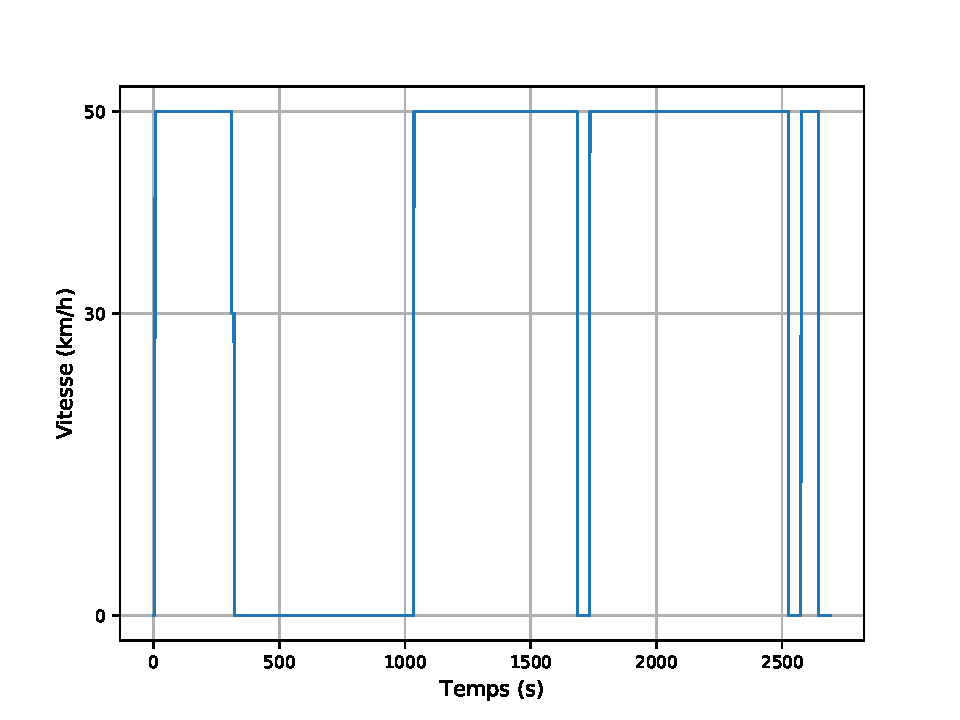
\includegraphics[width=\linewidth]{speed.pdf}  
    \caption{Évolution de la vitesse}
    \label{fig:speed}
\end{figure}

\subsection{Partitionnement CPU}

Les résultats obtenus s'observent à la figure~\ref{fig:partitionnement}, qui représente une simulation de 60 secondes.

On observe que la partition discrète consomme beaucoup plus que la partition continue. C'est normal, puisque la période de la partie discrète est 50 fois moins grande que celle des tâches de l'autre partition -- nécessaire afin d'accélérer la simulation.

On remarque également que la partition système consomme plus de ressources au début afin de créer les fils, créer les partitions et assigner les précédents fils aux partitions. Sa consommation pendant la simulation s'explique car les timers tournent toujours sur la partition système et d'autres processus tournent également sur l'OS en parallèle de notre programme.

\begin{figure}[h]
    \centering
    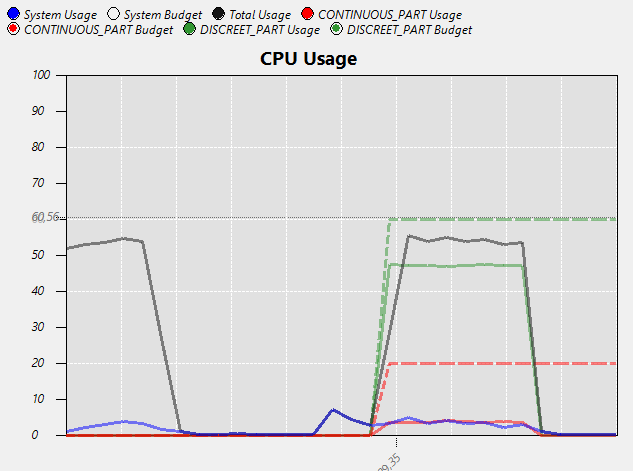
\includegraphics[width=\linewidth]{partitionnement.png}
    \caption{Partitionnement des tâches discrètes et continues}
    \label{fig:partitionnement}
\end{figure}

\section{Conclusion}

L'objectif de ce projet était d'implémenter le comportement de la voiture autonome modélisée depuis son commencement, en prenant en compte les enjeux du concept temps-réel. Ainsi, le système d'exploitation QNX a été employé à bon escient, avec l'utilisation de tous les outils tels que les sémaphores, mutexs et timers qui nous ont permis de répondre aux exigences temporelles du système. 

D'autre part, nous avions également pour objectif d'améliorer le système en termes de fonctionnalités et de performance. Parmi ces améliorations nous avons compté l'optimisation de l'utilisation des ressources CPU et mémoire du système ainsi que la modélisation correcte du comportement du système afin qu'il puisse faire face aux différentes situations possibles.

Nous pouvons dire que nous sommes parvenus dans un premier temps à apporter des solutions efficaces aux différents problèmes auxquels nous avons fait face dans la première étape du projet. Mais aussi, nous avons pu intégré des améliorations à notre travail qui permettent de représenter le fonctionnement de la voiture autonome de manière plus réaliste ainsi que d'optimiser l'implémentation du système.

La simulation, présentée dans cette article, témoigne de la performance du système, étant donné qu'elle a pu être exécutée de nombreuses fois avec facteur d'accélération assez important afin de garantir son bon fonctionnement sur un grand nombre de destinations atteintes. 

Enfin, nous notons que d'autres améliorations auraient pu être ajoutés à notre travail, telles que l'affinité des threads (qui consiste à lier chaque thread à un CPU spécifique, utilisé généralement pour palier aux erreurs de cache) ou encore l'intégration de \enquote{watchdogs} (procédé souvent utilisé dans le temps réel, il permet d'éviter le blocage du processus en cas d'erreur ou d'action malveillante en redémarrant le système notamment).

%\begin{thebibliography}{00}
%\bibitem{b1} G. Eason, B. Noble, and I. N. Sneddon, ``On certain integrals of Lipschitz-Hankel type involving products of Bessel functions,'' Phil. Trans. Roy. Soc. London, vol. A247, pp. 529--551, April 1955..
%\end{thebibliography}

\onecolumn

\appendix 

\lstinputlisting[language=python, caption=\lstname]{plot_data.py}

\begin{figure}[h!]
    \centering
    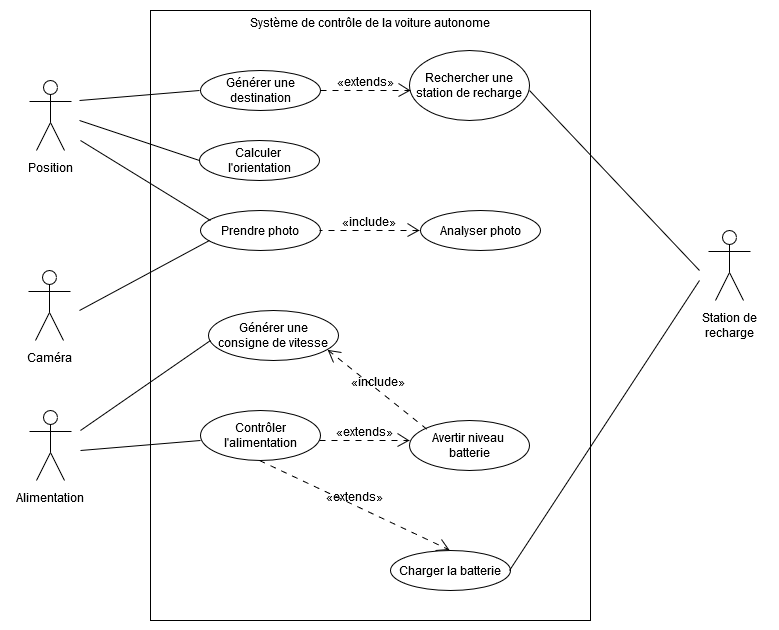
\includegraphics[width=\linewidth]{usecase.png}
    \caption{Diagramme de cas d'utilisation}
    \label{fig:usecase}
\end{figure}

\begin{figure}[h!]
    \centering
    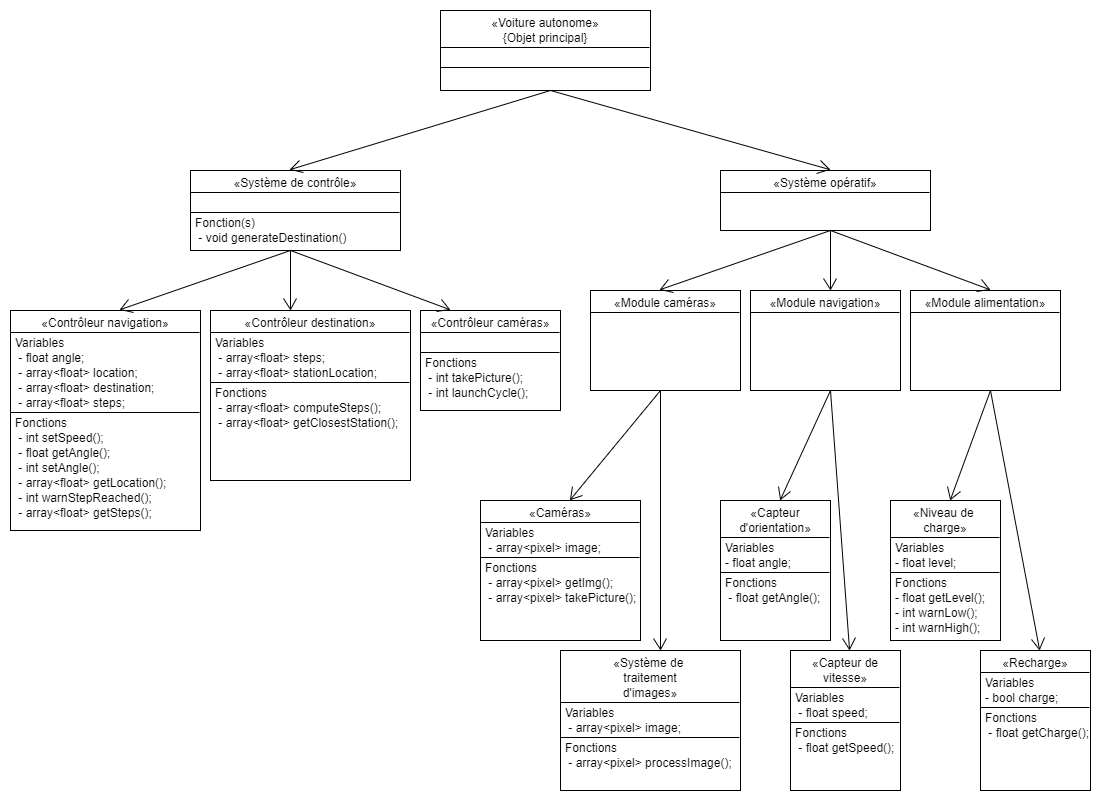
\includegraphics[width=\paperwidth, angle=90]{objects.png}
    \caption{Diagramme d'objets}
    \label{fig:object}
\end{figure}



\begin{figure}[h!]
    \hspace{-3em}
    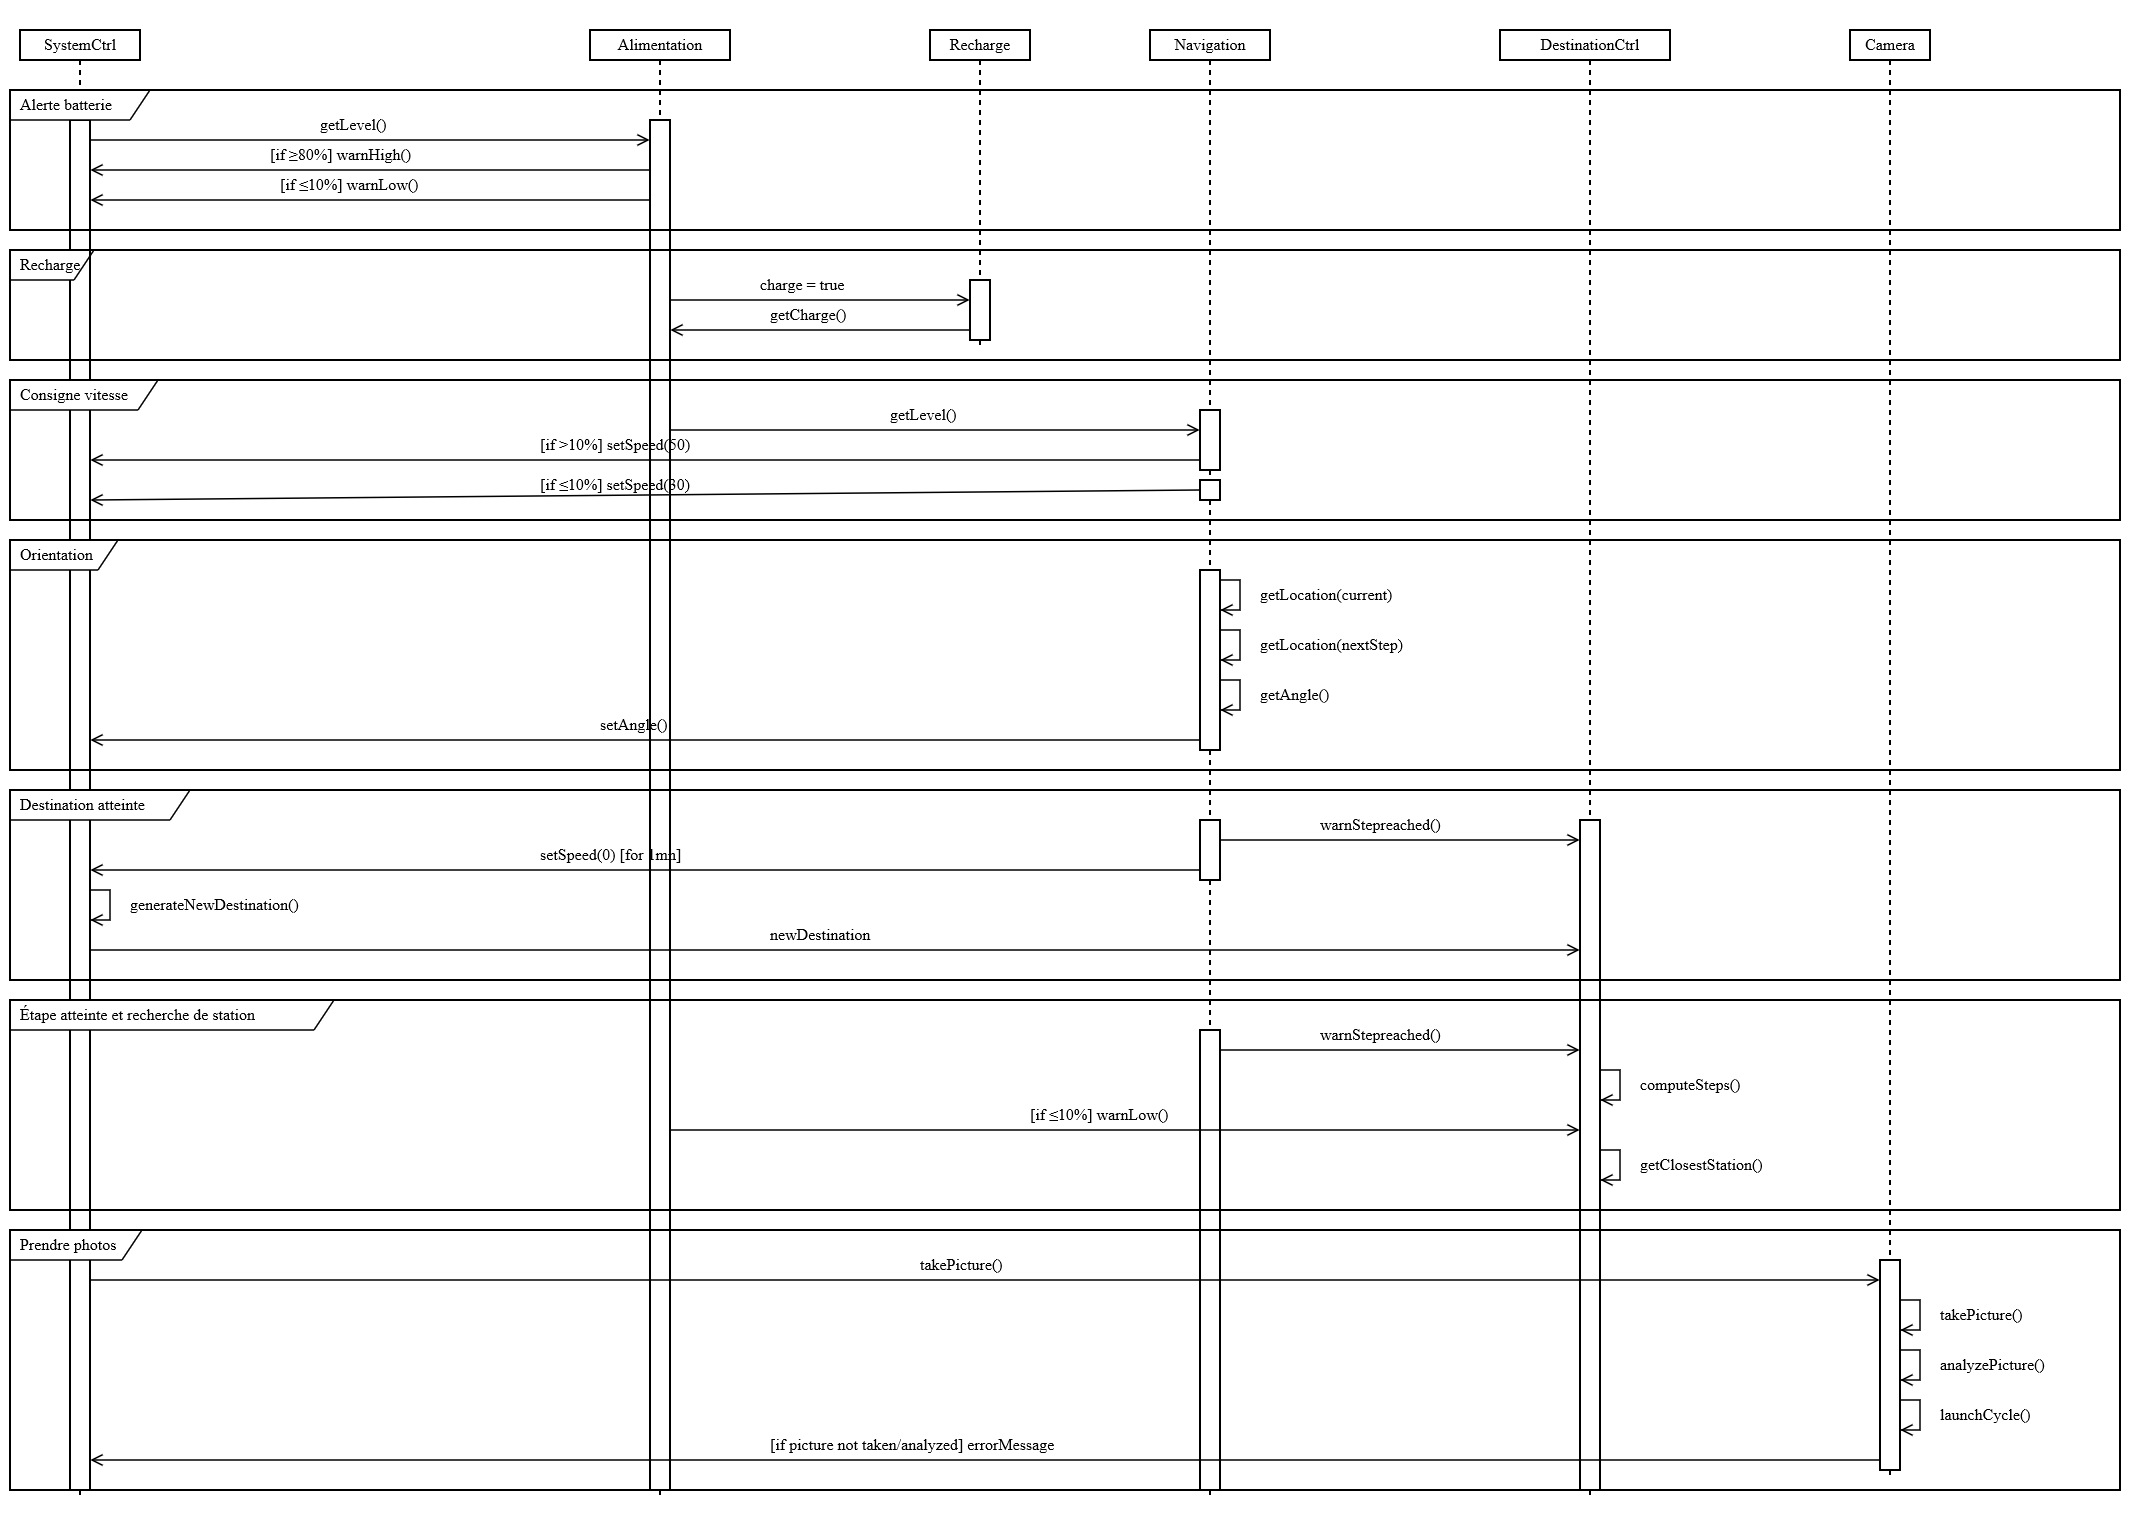
\includegraphics[width=1.2\paperwidth, angle=90]{sequence-diagram.png}
    \caption{Diagramme de séquence}
    \label{fig:sequence}
\end{figure}

\begin{figure}[h!]
    \hspace{-7em}
    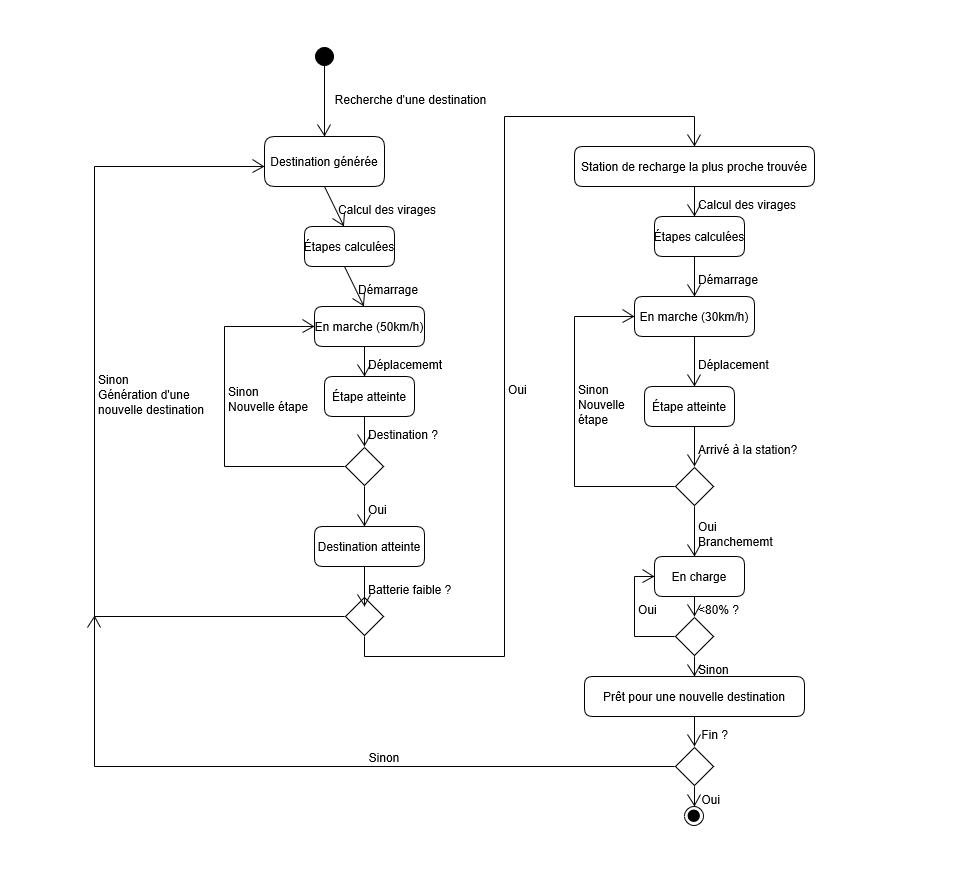
\includegraphics[width=1.35\linewidth]{activity.PNG}
    \caption{Diagramme d'activitité}
    \label{fig:activity}
\end{figure}


\end{document}